\documentclass{standalone}

\usepackage[utf8]{inputenc}
\usepackage[no-math]{fontspec}

\usepackage{graphicx}
\usepackage{tikz}
\usetikzlibrary{shapes,decorations.pathreplacing,calligraphy,positioning,shadows,fit,calc,arrows.meta}
\usepackage{color}
\usepackage{xcolor}

\definecolor{lgray}{RGB}{200,199,200}
\definecolor{lblue}{RGB}{191,207,238}
\definecolor{rwthblue}{RGB}{23,111,193}
\definecolor{rwthred}{RGB}{210,32,39}

\setmainfont{HelveticaNeueLTStd-Cn.otf}[Path=/home/denes/fonts/from_csilla/, BoldFont=HelveticaNeueLTStd-MdCn.otf]

%\pgfkeys{/cclwd/Dendritic cell/Goblet cell}

\begin{document}

    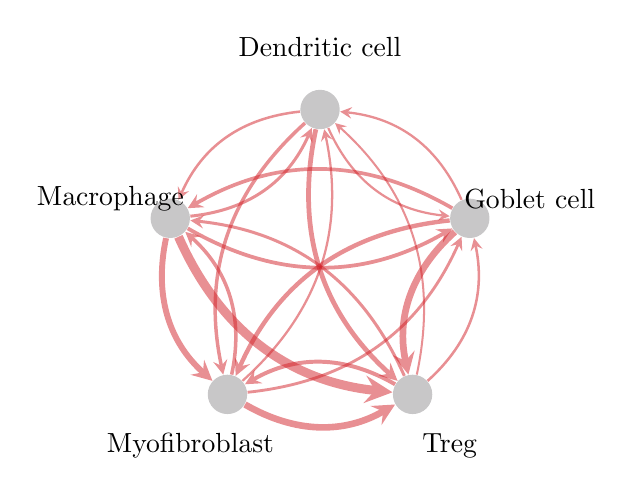
\begin{tikzpicture}[cell/.style={circle, fill=lgray, minimum width=5mm, inner sep=2pt}]

        \foreach \lab [count=\c, evaluate=\c as \ang using {18+72*\c}]
            in {Dendritic cell, Macrophage, Myofibroblast, Treg, Goblet cell} {
                \node[cell] (\lab) at (\ang:20mm) {};

        }

        \begin{scope}[
            every path/.style={->,>=stealth,draw=rwthred},
            every to/.style={bend right}
        ]

            \begin{scope}[opacity=.5, transparency group]\path[line width=1.25pt](Dendritic cell) to (Myofibroblast);\end{scope}
            \begin{scope}[opacity=.5, transparency group]\path[line width=0.91pt](Dendritic cell) to (Macrophage);\end{scope}
            \begin{scope}[opacity=.5, transparency group]\path[line width=0.795pt](Dendritic cell) to (Goblet cell);\end{scope}
            \begin{scope}[opacity=.5, transparency group]\path[line width=1.715pt](Dendritic cell) to (Treg);\end{scope}

            \begin{scope}[opacity=.5, transparency group]\path[line width=0.82pt](Myofibroblast) to (Dendritic cell);\end{scope}
            \begin{scope}[opacity=.5, transparency group]\path[line width=1.27pt](Myofibroblast) to (Macrophage);\end{scope}
            \begin{scope}[opacity=.5, transparency group]\path[line width=1.03pt](Myofibroblast) to (Goblet cell);\end{scope}
            \begin{scope}[opacity=.5, transparency group]\path[line width=2.39pt](Myofibroblast) to (Treg);\end{scope}

            \begin{scope}[opacity=.5, transparency group]\path[line width=0.73pt](Treg) to (Dendritic cell);\end{scope}
            \begin{scope}[opacity=.5, transparency group]\path[line width=1.085pt](Treg) to (Macrophage);\end{scope}
            \begin{scope}[opacity=.5, transparency group]\path[line width=0.915pt](Treg) to (Goblet cell);\end{scope}
            \begin{scope}[opacity=.5, transparency group]\path[line width=1.43pt](Treg) to (Myofibroblast);\end{scope}

            \begin{scope}[opacity=.5, transparency group]\path[line width=0.83pt](Goblet cell) to (Dendritic cell);\end{scope}
            \begin{scope}[opacity=.5, transparency group]\path[line width=1.33pt](Goblet cell) to (Macrophage);\end{scope}
            \begin{scope}[opacity=.5, transparency group]\path[line width=2.43pt](Goblet cell) to (Treg);\end{scope}
            \begin{scope}[opacity=.5, transparency group]\path[line width=1.58pt](Goblet cell) to (Myofibroblast);\end{scope}

            \begin{scope}[opacity=.5, transparency group]\path[line width=1.09pt](Macrophage) to (Dendritic cell);\end{scope}
            \begin{scope}[opacity=.5, transparency group]\path[line width=1.36pt](Macrophage) to (Goblet cell);\end{scope}
            \begin{scope}[opacity=.5, transparency group]\path[line width=3.26pt](Macrophage) to (Treg);\end{scope}
            \begin{scope}[opacity=.5, transparency group]\path[line width=2.14pt](Macrophage) to (Myofibroblast);\end{scope}

        \end{scope}

        \foreach \lab [count=\c, evaluate=\c as \ang using {18+72*\c}]
        in {Dendritic cell, Macrophage, Myofibroblast, Treg, Goblet cell} {
            \node at (\ang:28mm){\lab};

        }

    \end{tikzpicture}

\end{document}